%!TEX root=paper/thesis.tex
\section{Problem Definition}\label{sec:clf_problem}

\begin{mydef} \label{def:clf_problem}
\textbf{The test-time efficient multi-class classification problem} consists of

\begin{itemize}
    \item $N$ instances labeled with one of $K$ labels: ${\mathcal{D} = \{x_n \in \mathcal{X}, y_n \in \mathcal{Y} = \{1, \dots, K\}\}_{n=1}^N}$.
    \item $F$ features $\mathcal{H} = \{h_f : \mathcal{X} \mapsto \mathbb{R}^{d_f} \}_{f=1}^F$, with associated costs $c_f$.
    \item Budget-sensitive loss $\mathcal{L}_\mathcal{B}$, composed of cost budget $\mathcal{B}$ and loss function ${\ell(\hat{y}, y) \mapsto \mathbb{R}}$.
\end{itemize}

The goal is to find a \textbf{feature selection} policy $\pi(x): \mathcal{X} \mapsto 2^\mathcal{H}$ and a \textbf{feature combination} classifier $g(\mathcal{H}_\pi) : 2^\mathcal{H} \mapsto \mathcal{Y}$ such that such that the total budget-sensitive loss $\sum \mathcal{L}_\mathcal{B}(g(\pi(x_n)), y_n)$ is minimized.
\end{mydef}

\PM{Budget}
The cost of a selected feature subset $\mathcal{H}_{\pi(x)}$ is $C_{\mathcal{H}_\pi(x)}$.
The budget-sensitive loss $\mathcal{L}_\mathcal{B}$ presents a hard budget constraint by only accepting answers with $C_{\mathcal{H}} \leq \mathcal{B}$.
Additionally, $\mathcal{L}_\mathcal{B}$ can be \textbf{cost-sensitive}: answers given with less cost are more valuable than costlier answers.
As discussed in \autoref{sec:introduction}, the motivation for the latter property is Anytime performance; we should be able to stop our algorithm's execution at any time and have the best possible answer.

\PM{Cost}
Feature costs $c_f$ can be specified flexibly, with options including theoretical analysis, number of flops, wall clock runtime, total CPU time, or exact power expenditure.
We believe that a deployment in a modern datacenter is most likely to optimize for power expenditure.
In the absence of reliable ways to measure power, we use total CPU time to define the cost: if an operation is performed in parallel on multiple cores, its cost is considered to be the total cpu time on all cores.

\PM{Shared features}
The features $h_f$ can be classifier outputs, possibly multi-class; following convention, we refer to such features as \emph{weak learners}.
For a weak learner $h_f$, the cost $c_f$ is composed of the cost of an underlying feature extraction $\phi_{h_f}(x)$ and the cost of subsequent classification.
Once $h_f$ is computed, its underlying feature $\phi$ is considered to be free for all other features $h_f'$ that share it, if any, such that $c_f' < c_f$.
Note that in state-of-the-art object recognition systems, complex features and feature encodings are often followed by linear classifiers, and feature extraction cost dominates the total cost.

\begin{figure}[ht]
\centering
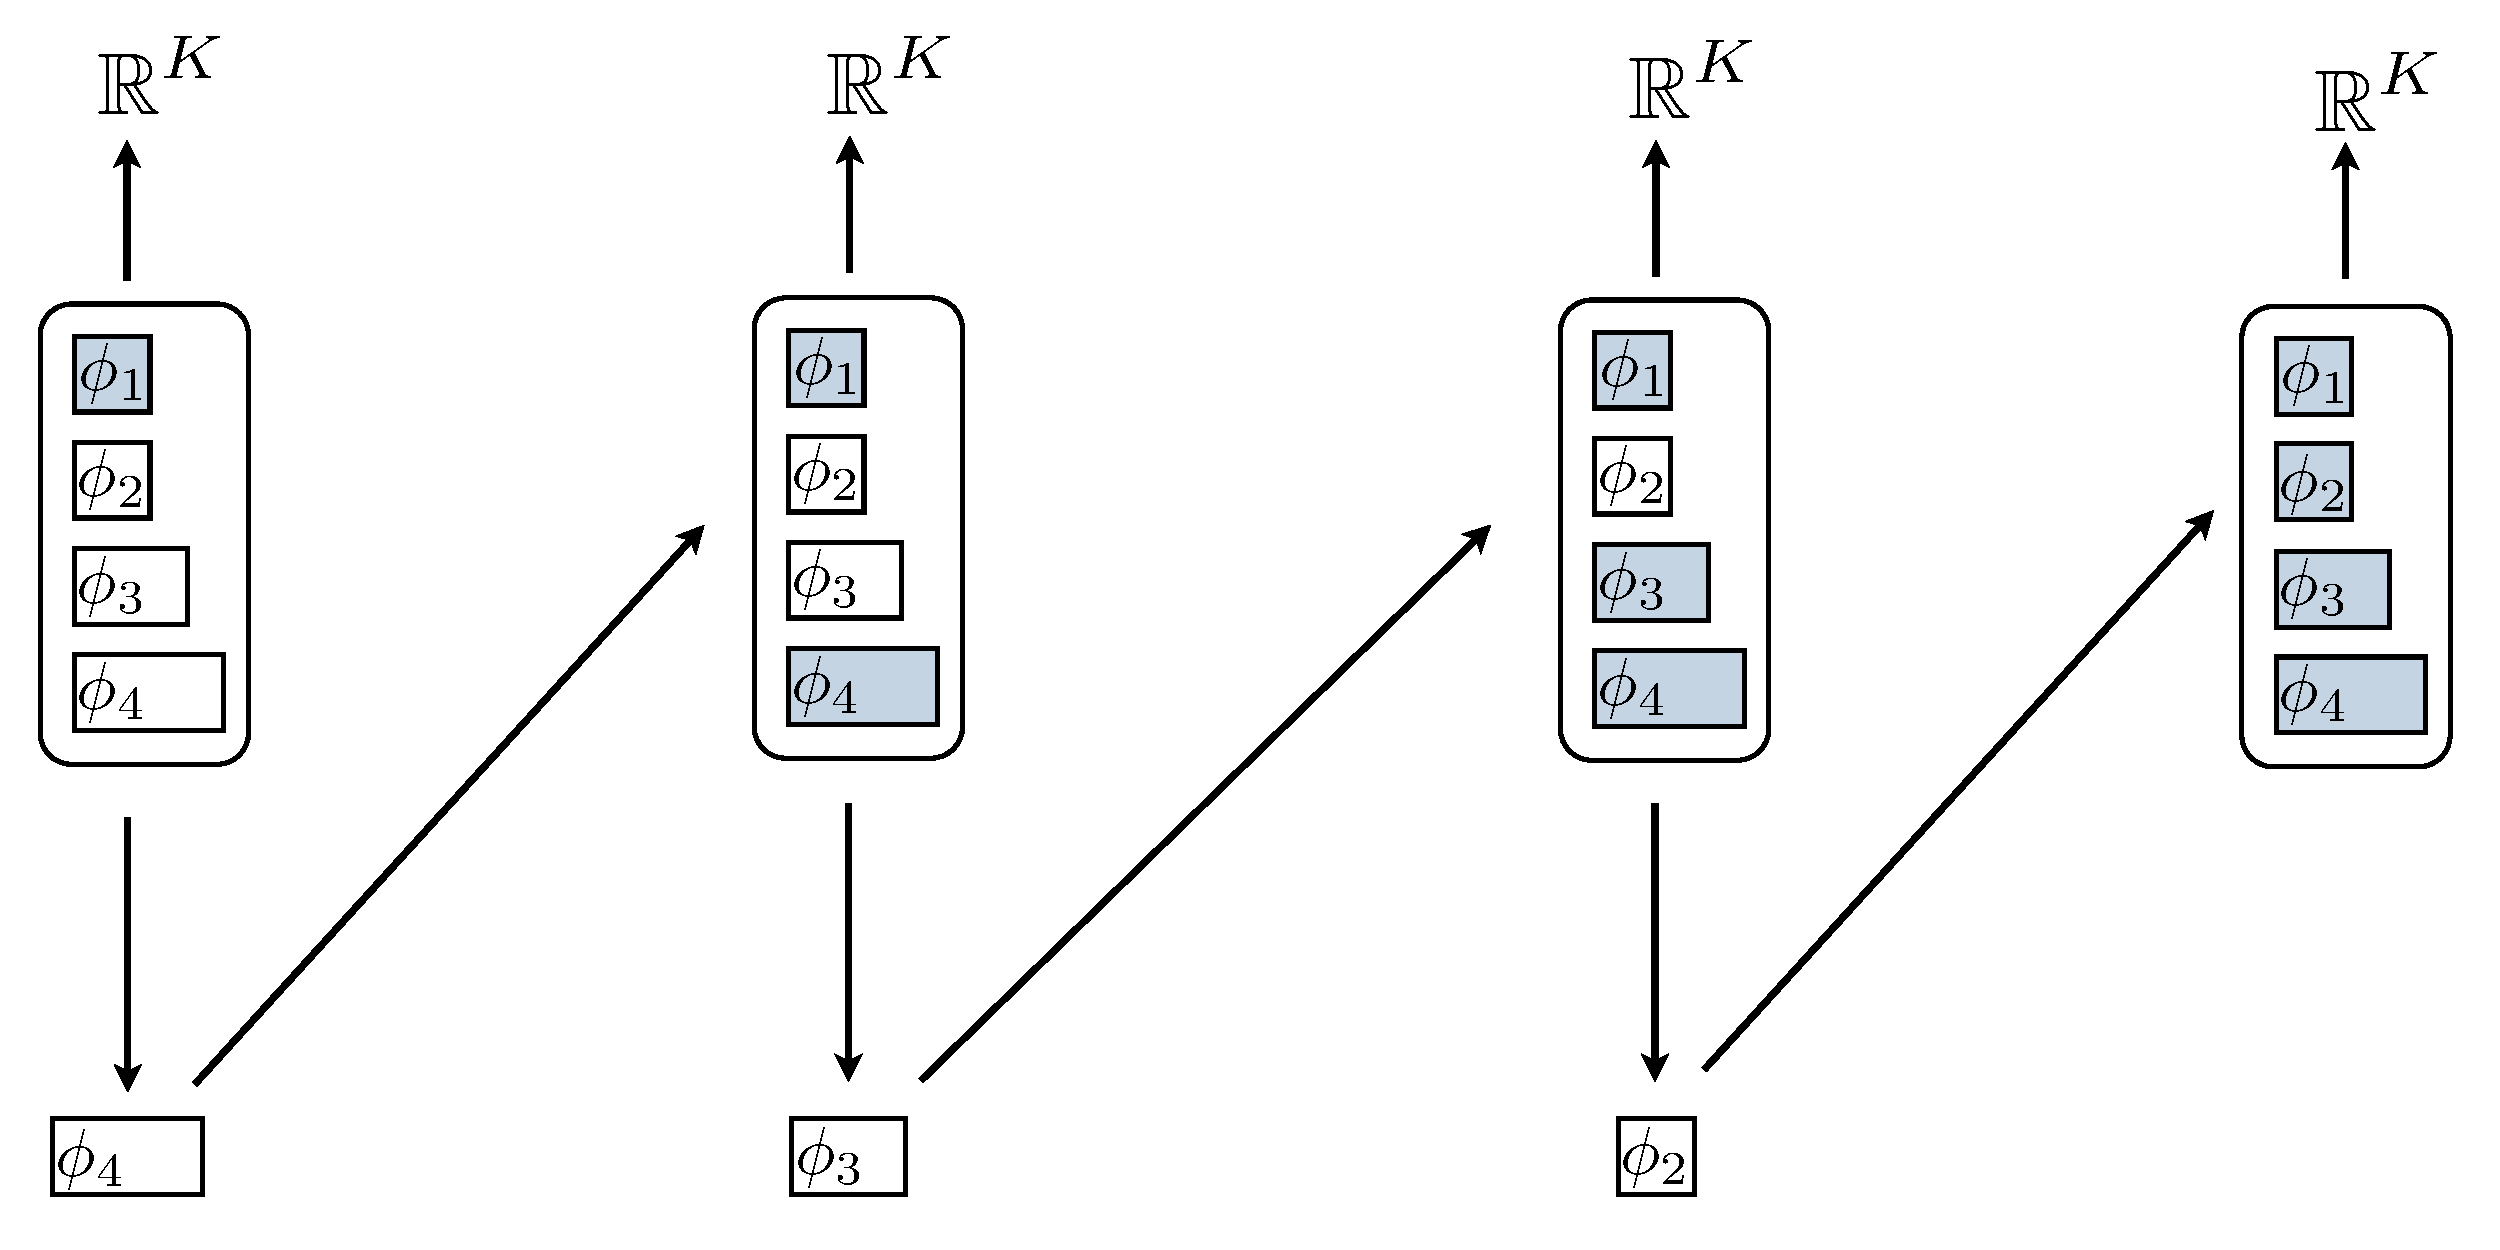
\includegraphics[width=.85\linewidth]{../../figures/feature_selection_sequence.pdf}
\caption[
Summary of our dynamic feature selection approach to the classification problem.]{
We model the problem of state traversal as a Markov Decision Process.
For every state, we learn to select action of maximum expected value.
The state is updated with the result of the selected action.
We train a classifier on subsets of features, to give answer at any time.
}\label{fig:feature_selection_sequence}
\end{figure}


\PM{Train vs. Test}
At training time, our computation is unbudgeted, and we can compute all features to have \emph{fully-observed} training instances.
At test time, there is a budget and so the instances we classify will only be \emph{partially-observed}, as determined by the feature selection policy.
\autoref{fig:feature_selection_sequence} shows the sequential process we are learning.
